 \let\negmedspace\undefined
\let\negthickspace\undefined
\documentclass[journal]{IEEEtran}
\usepackage[a5paper, margin=10mm, onecolumn]{geometry}
%\usepackage{lmodern} % Ensure lmodern is loaded for pdflatex
\usepackage{tfrupee} % Include tfrupee package

\setlength{\headheight}{1cm} % Set the height of the header box
\setlength{\headsep}{0mm}     % Set the distance between the header box and the top of the text
\usepackage{gvv-book}
\usepackage{gvv}
\usepackage{cite}
\usepackage{amsmath,amssymb,amsfonts,amsthm}
\usepackage{algorithmic}
\usepackage{graphicx}
\usepackage{textcomp}
\usepackage{xcolor}
\usepackage{txfonts}
\usepackage{listings}
\usepackage{enumitem}
\usepackage{mathtools}
\usepackage{gensymb}
\usepackage{comment}
\usepackage[breaklinks=true]{hyperref}
\usepackage{tkz-euclide} 
\usepackage{listings}
% \usepackage{gvv}                                        
\def\inputGnumericTable{}                                 
\usepackage[latin1]{inputenc}                                
\usepackage{color}                                            
\usepackage{array}                                            
\usepackage{longtable}                                       
\usepackage{calc}                                             
\usepackage{multirow}                                         
\usepackage{hhline}                                           
\usepackage{ifthen}                                           
\usepackage{lscape}



\usepackage{amsmath,amssymb}
\usepackage{booktabs}
\usepackage{tikz}
\usetikzlibrary{arrows.meta,angles,quotes}





\begin{document}

\bibliographystyle{IEEEtran}
\vspace{3cm}

\title{4.8.17}
\author{AI25BTECH11021 - Abhiram Reddy N}
% \maketitle
% \newpage
% \bigskip
{\let\newpage\relax\maketitle}

\renewcommand{\thefigure}{\theenumi}
\renewcommand{\thetable}{\theenumi}
\setlength{\intextsep}{10pt} % Space between text and floats


\numberwithin{equation}{enumi}
\numberwithin{figure}{enumi}
\renewcommand{\thetable}{\theenumi}


\section*{Question}
The foot of a perpendicular drawn from the point \((-2, -1, -3)\) on a plane is \((1, -3, 3)\). Find the equation of the plane.

\section*{Answer}

\subsection*{\textbf{Step 1}: Understanding the problem}
Given:
\[
\vec{P} = \begin{pmatrix} -2 \\ -1 \\ -3 \end{pmatrix}, \quad
\vec{F} = \begin{pmatrix} 1 \\ -3 \\ 3 \end{pmatrix}
\]
where \(\vec{P}\) is the point from which the perpendicular is dropped and \(\vec{F}\) is the foot of the perpendicular on the plane.

\subsection*{\textbf{Step 2}: Vector along the perpendicular}
The vector along the perpendicular from \(\vec{P}\) to \(\vec{F}\) is:
\[
\vec{P}\vec{F} = \vec{F} - \vec{P} = \begin{pmatrix} 1 \\ -3 \\ 3 \end{pmatrix} - \begin{pmatrix} -2 \\ -1 \\ -3 \end{pmatrix} = \begin{pmatrix} 3 \\ -2 \\ 6 \end{pmatrix}
\]

\subsection*{\textbf{Step 3}: Normal vector to the plane}
Since the perpendicular from \(\vec{P}\) to the plane hits the foot \(\vec{F}\), the vector \(\vec{P}\vec{F}\) is normal to the plane. Therefore, the normal vector to the plane \(\vec{n}\) is:
\[
\vec{n} = \vec{P}\vec{F} = \begin{pmatrix} 3 \\ -2 \\ 6 \end{pmatrix}
\]

\subsection*{\textbf{Step 4}: Equation of the plane in vector form}
The vector form of the plane equation is:
\[
\vec{n}^T (\vec{r} - \vec{F}) = 0
\]
where \(\vec{r} = \begin{pmatrix} x \\ y \\ z \end{pmatrix}\) is any point on the plane.

\subsection*{\textbf{Step 5}: Substitute values and expand}
Substituting \(\vec{n}\) and \(\vec{F}\):
\[
\begin{pmatrix} 3 & -2 & 6 \end{pmatrix} \left( \begin{pmatrix} x \\ y \\ z \end{pmatrix} - \begin{pmatrix} 1 \\ -3 \\ 3 \end{pmatrix} \right) = 0
\]

\[
\Rightarrow \begin{pmatrix} 3 & -2 & 6 \end{pmatrix} \begin{pmatrix} x-1 \\ y+3 \\ z-3 \end{pmatrix} = 0
\]

\[
3(x-1) - 2(y+3) + 6(z-3) = 0
\]

\subsection*{\textbf{Step 6}: Simplify the equation}
\[
3x - 3 - 2y - 6 + 6z - 18 = 0
\]

\[
3x - 2y + 6z - 27 = 0
\]

\subsection*{\textbf{Final answer:}}
\[
\boxed{3x - 2y + 6z = 27}
\]


\begin{figure}[htbp]
\centering
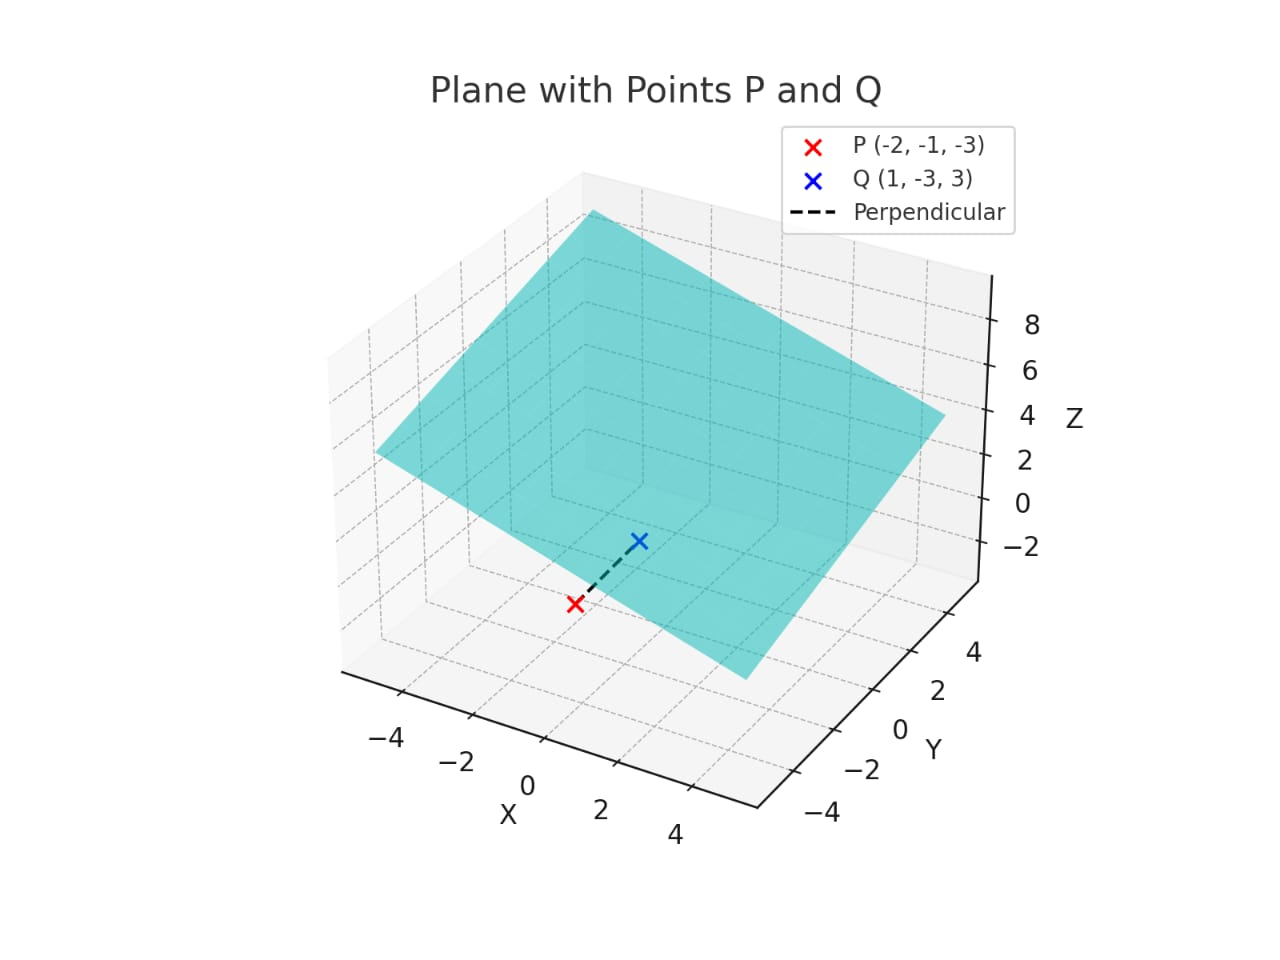
\includegraphics[width=0.8\columnwidth]{figs/python_plot.png} 
\caption*{Plot of the points and plane with perpendicular.}
\label*{fig:1}
\end{figure}


\end{document}